\section{Daten}
\label{sec:daten}
In diesem Abschnitt wird gezeigt was für Daten vom Öffentlichen Verkehr auf der Plattform\footnote{\url{https://opentransportdata.swiss/}} zur Verfügung stehen. Anschliessend werden die Datenformate vorgestellt und analysiert. Die Fahrplandaten werden in zwei verschiedenen Formaten bereitgestellt GTFS und HRDF. 

\subsection{Fahrplan General Transit Feed Specification (GTFS)}
\label{sec:gtfs-static}
General Transit Feed Specification (GTFS) ist ein von Google entwickeltes Dateiformat zum Austausch von Öffentlichen Verkehrsdaten sprich Fahrpläne. Ursprünglich wurde es Google Transit Feed Specification (GTFS) genannt (bis 2010), weil es ausschliesslich für Google Maps genutzt wurde. Dies änderte sich aber mit der Zeit sehr stark da viele neue Applikationen herauskamen die diese Daten verwendeten die nicht von Google waren und somit änderte man den Namen zu General Transit Feed Specification (GTFS).\cite{gtfsbackground}
\newline
GTFS beinhaltet nicht nur Informationen über Fahrpläne sondern auch über Geographische Orte wie Haltestellen. GTFS ist ein statisches Dateiformat und beinhaltet keine Echtzeitdaten deshalb wird es auch GTFS Static genannt.\cite{gtfs}

\subsubsection{Datenstruktur}
\label{sec:gtfs-datenstruktur}
Die GTFS Datei besteht aus nichts anderen als Textfiles, die durch Datenfelder(Werte) und Kommas getrennt sind, dieses Format nennt man auch Comma-Separated Values (CSV).

\begin{figure}[]
	\centering
	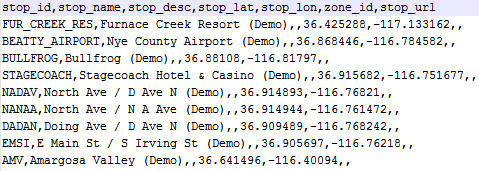
\includegraphics[width=8cm]{bspcsv.png}
	\caption{Hier sieht man wie so ein CSV-Format im Texteditor aussieht.}
	\label{fig:gtfs-dateiformat}
\end{figure}

Die verschiedenen Textfiles decken viele wichtige Informationen ab, die für ein GTFS benötigt werden.

\begin{tabular}{|l|c|l|}  \hline
	Dateiname & pflicht? & Definition \\ \hline
	agency.txt & ja & Geschäftsstellen die Daten zur Verfügung stellen \\ \hline
	stops.txt & ja & Haltestellen mit ihrer Position \\ \hline
	routes.txt & ja & Verkehrsverbindungen (Linien) mit den Fahrzeugarten \\ \hline %(zeitunabhängig)
	trips.txt & ja & Fahrten  \\ \hline												%(zeitabhängig)
	stop\_times.txt & ja & Zeiten in der Fahrzeuge Ankommen/Abfahren an Haltestellen \\ \hline
	calendar.txt & ja & Fahrplanveränderungen (Jahreszeiten) \\ \hline
	calendar\_dates & optional & Ausnahmeplan für bestimmtes Datum \\ \hline
	fare\_attributes.txt & optional & Fahrpreise und die Art der Bezahlung \\ \hline
	fare\_rules.txt & optional & Fahrpreisregeln verschiedener Zonen  \\ \hline
	shapes.txt & optional & Beschreibt den Weg eines Fahrzeuges (Darstellung) \\ \hline
	frequencies.txt & optional & Fahrpläne ohne fixe stop Zeiten. \\ \hline
	transfers.txt & optional & Umsteigpunkte verschiedener Routen (Linien) \\ \hline
	feed\_info.txt & optional & Zusätzliche Informationen über den Datensatz \\ \hline	
\end{tabular}
\cite{gtfsInhalt}
Daten die bisher nicht von der Plattform zur Verfügung gestellt werden: fare\_attributes.txt, fare\_rules.txt, frequencies.txt. 

\begin{figure}[]
	\centering
	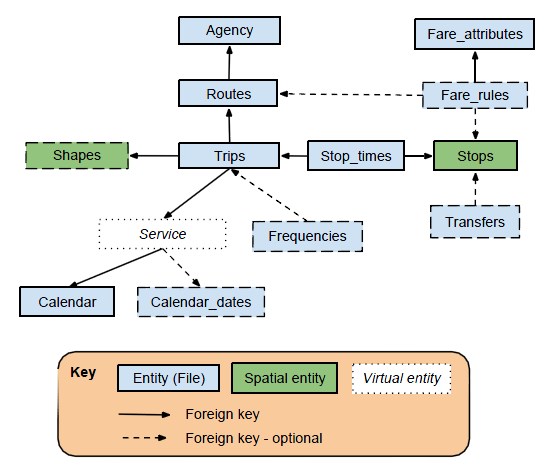
\includegraphics[scale=0.75]{GTFS_data_model_diagram.png}
 	\caption{Diese Übersicht zeigt die Abhängigkeiten der einzelnen Files.z.B. Braucht das Trips-File die Info der Route-Files(route\_id) um zu wissen auf welchem Weg diese Reise stattfindet.  \cite{gtfsUebersicht}}
	\label{fig:gtfs-uebersicht}
\end{figure}

 

\subsubsection{Vor- und Nachteile}
\label{sec:gtfs-vornachteile}
Die Daten können einfach von Mensch und Maschine gelesen werden, wegen dem einfachen Aufbau der Textfiles. Zudem stellt Google hierfür eine sehr gute Anleitung zur Verfügung, wie diese Daten verwendet werden und aufgebaut sind.

\subsection{GTFS Realtime (GTFS-RT)}
\label{sec:gtfs-rt}
GTFS-RT ist eine Erweiterung der GTFS-Static Daten. Wie der Name Realtime schon sagt handelt sich hier um Echtzeitdaten. 
\subsubsection{Datenstruktur}
\label{sec:gtfs-rt-datenstruktur}
GTFS-RT stellt folgende Daten zusätzlich in diesem Format zur Verfügung. Die Daten werden geschrieben/gelesen basierend auf sogenannten "Protocol Buffers", die stehen in vielen Programmiersprachen zur Verfügung (C++,C, Go, Java, Python).\cite{gtfs-rt}
\begin{itemize}
	\item{\textbf{Trip Updates}} -Hier werden Aktuelle Verspätungen, geänderte Routen, Ersatzfahrzeuge oder Ausfälle publiziert.  
	\item{\textbf{Service Alerts}} -Hier werden Informationen über Probleme mit Stationen,  Linien, das Ganze Netzwerk etc. übermittelt. 
	\item{\textbf{Vehicle Positions}} -Hier werden Daten geliefert die eine genaue Position des Vehicles mit der dazugehörigen Zeit liefert.\cite{gtfs-rt-google} 
\end{itemize}


\subsubsection{Vor- und Nachteile}
\label{sec:gtfs-rt-vornachteile}
Google stellt auch hier eine Gute Übersichtliche Anleitung zur Verwendung von GTFS-RT zur Verfügung.

\subsection{Fahrplan Hafas Rohdaten Format (HRDF)}
\label{subsec:hrdf}
Neben GTFS ist HRDF ein weiteres Dateiformat das die Fahrplandaten zur Verfügung stellt. 
Dieses Dateiformat kommt von der Firma HaCon. Das Format wird für ihren eigenen Journey Planner (HaCon Fahrplan-Auskunfts-System (HAFAS)) genutzt. Zudem stellt HaCon eine Plannungssoftware (Train Planning System TPS) für Infrastrukturbetreiber (wie Eisenbahnverkehrsunternehmen usw.) zur Verfügung. HRDF ist somit ihr eigenes Datenaustauschformat von Fahrplandaten.\cite{haconUebersicht}


\begin{figure}[]
	\centering
	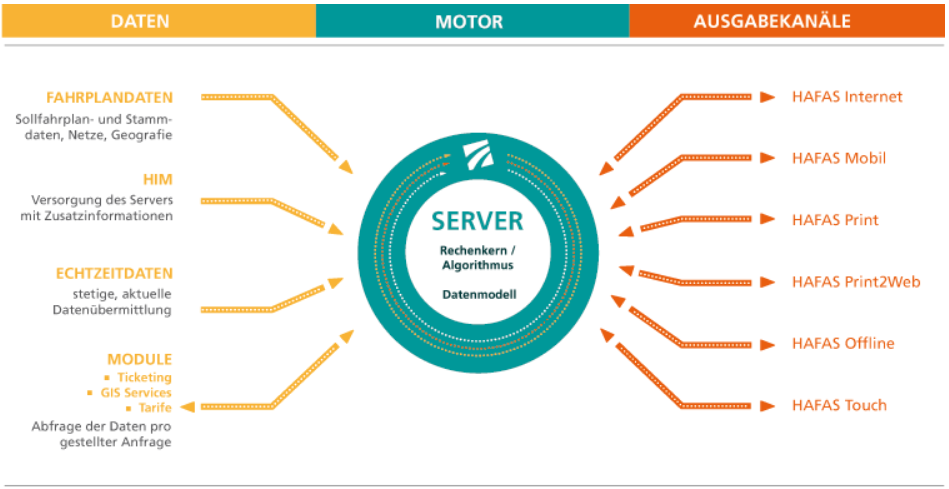
\includegraphics[width=12cm]{HAFAS.png}
	\caption{Dies ist eine Übersicht wie das HAFAS System aufgebaut ist. Die Fahrplandaten entsprechen hier dem HRDF-Format. \cite{haconUebersicht}}
	\label{fig:hafas-uebersicht}
\end{figure}



\subsubsection{Datenstruktur}
\label{sec:hrdf-datenstrukur}
Ähnlich wie GTFS-Files sind auch HRDF-Files auch Textfiles aber mit dem Unterschied das die Werte im Stil Tab-separated values (TSV) angelegt sind. Die Struktur der Daten ist etwas anders und um einiges komplizierter als bei GTFS. Auch sind die Daten oft schwerer zu lesen von Auge, weil sie manchmal als Bitfeld abgelegt sind. Nebenbei können HRDF Daten auch in GTFS-Daten konvertiert werden.\cite{hrdfintogtfs}
\begin{figure}[]
	\centering
	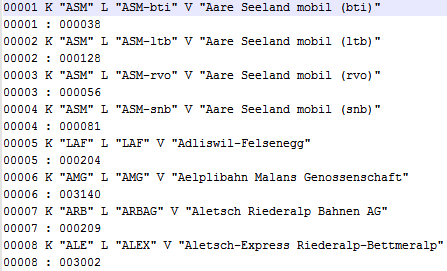
\includegraphics[width=8cm]{bsptsv.png}
	\caption{Hier sieht man wie so ein TSV-Format im Texteditor aussieht.}
	\label{fig:hrdf-dateiformat}
\end{figure}


\subsubsection{Vor- und Nachteile}	
\label{sec:hrdf-vornachteile}
Die Plattform warnt vor Verwendung der HRDF-Daten: "Die HRDF-Datei(en) sind relativ komplex. Ohne Not sollte nicht damit gearbeitet werden."\cite{opentransporthrdf}

\subsection{Fahrplan Überblick (timetable overview)}
\label{sec:Fahrplan Ueberblick}
Die Datei enthält alle Informationen der vorhandenen Fahrplandaten. Zusätzlich wird das Format(HRDF/GTFS) der Status, Gültigkeit und den Permalink der Fahrplandaten zur Verfügung gestellt.

\begin{figure}[]
	\centering
	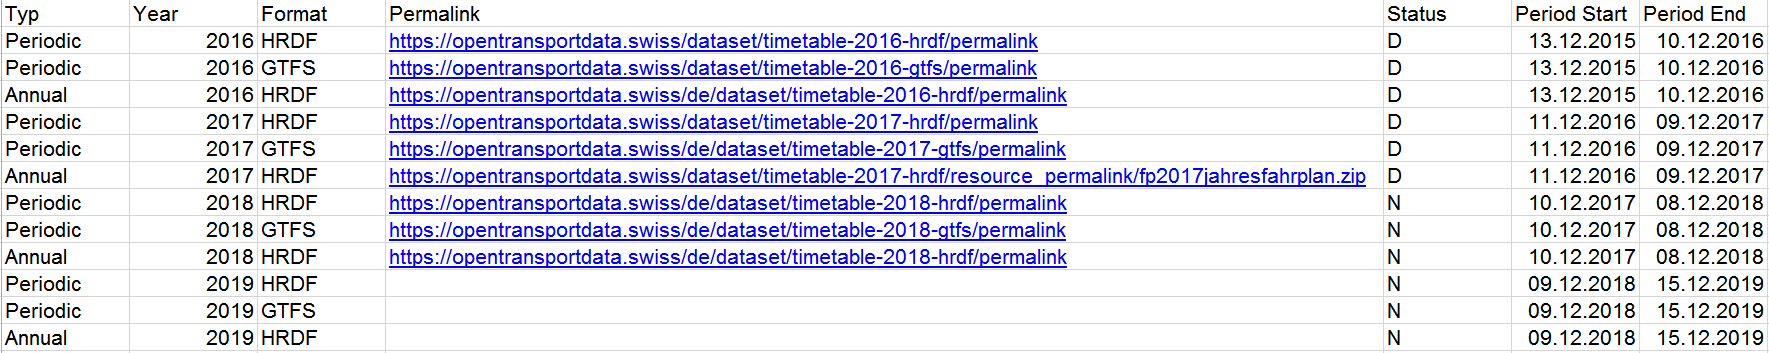
\includegraphics[width=12cm]{fahrplanueberblick.png}
	\caption{Die Fahrplan Überblick Datei wird hier in einer Excel Tabelle zur Verfügung gestellt.}
	\label{fig:Fahrplan Ueberblick dateiformat}
\end{figure}

\subsection{Ist-Daten (actual data)}
\label{sec:istdaten}
Bei den Ist-Daten handelt es sich um eine Ansammlung von Daten, welche die effektive gefahrenen Fahrten des letzten Tages enthalten. Somit sind diese Daten eigentlich in dem Sinne keine wirklichen Ist-Daten. Diese Daten können aber durchaus interessant sein für Statistiken:\cite{istdaten}
\begin{itemize}
	\item{Pünktlichkeit}   
	\item{Regelmässigkeit}. 
	\item{Anschlussqualität}  
\end{itemize}
Die Daten werden im CSV-Format bereitgestellt.

\subsection{Dienststellendokumentation (DiDok)}
\label{sec:didok}
Bei dieser Dokumentation geht es um die Daten zur Verwaltung der Stammdaten aller Dienststellen(Haltestellen) des öffentlichen Verkehrs der Schweiz. In dem Format werden Daten wie offizieller Name einer Haltestelle und die dazugehörige verantwortliche Geschäftsorganisation. Es werden aber auch die geographischen Koordinaten der Haltestellen mitgeliefert. Die Datei wird im Excel Format zur Verfügung gestellt.Die DiDok Daten werden vom BAV(Bundesamt für Verkehr) veröffentlicht. \cite{didok}

\begin{figure}[]
	\centering
	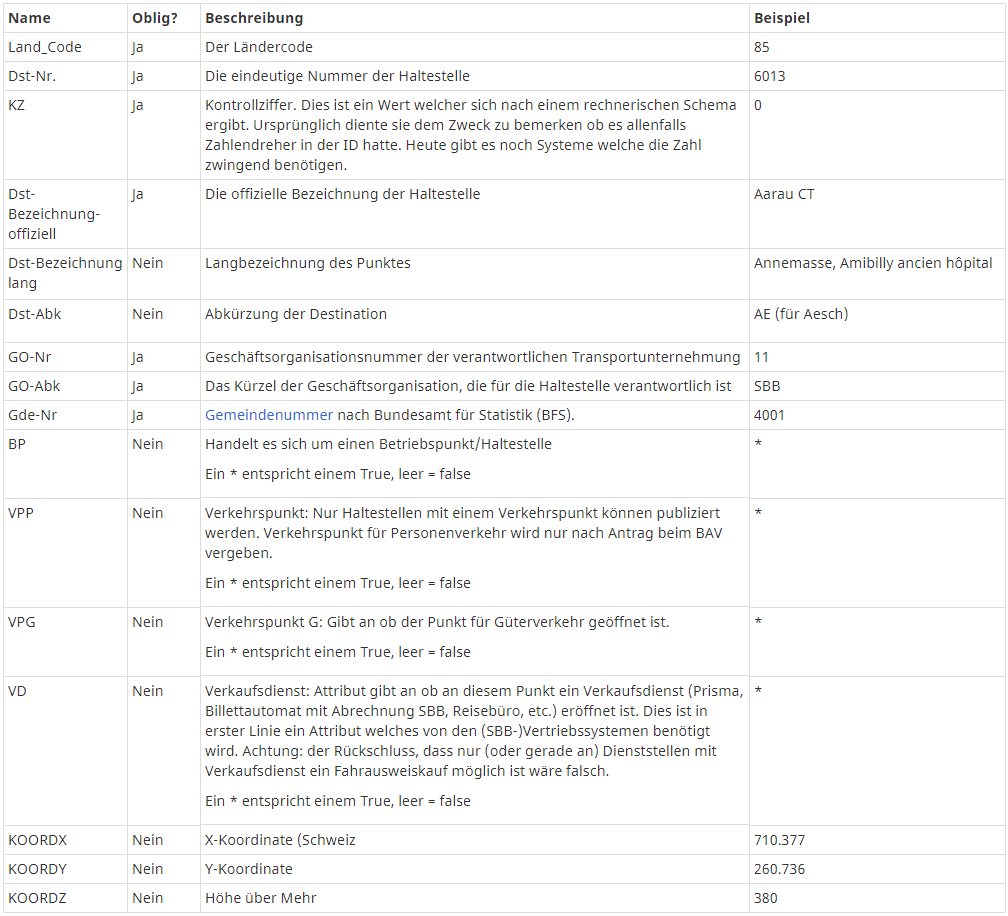
\includegraphics[width=15cm]{didokuebersicht.png}
	\caption{Hier sieht man ein Beispiel(Haltestelle) für das DiDok-File inklusive der Beschreibung einzelner Attribute.\cite{didok}}
	\label{fig:didok-uebersicht}
\end{figure}

\subsection{Geschäftsorganisationen (business organisations)}
\label{Geschaeftsorganisationen}
Die Daten werden im Excel-Format zur Verfügung gestellt. Hierbei findet man alle in der Schweiz operierenden Geschäftsorganisationen.
\begin{figure}[]
	\centering
	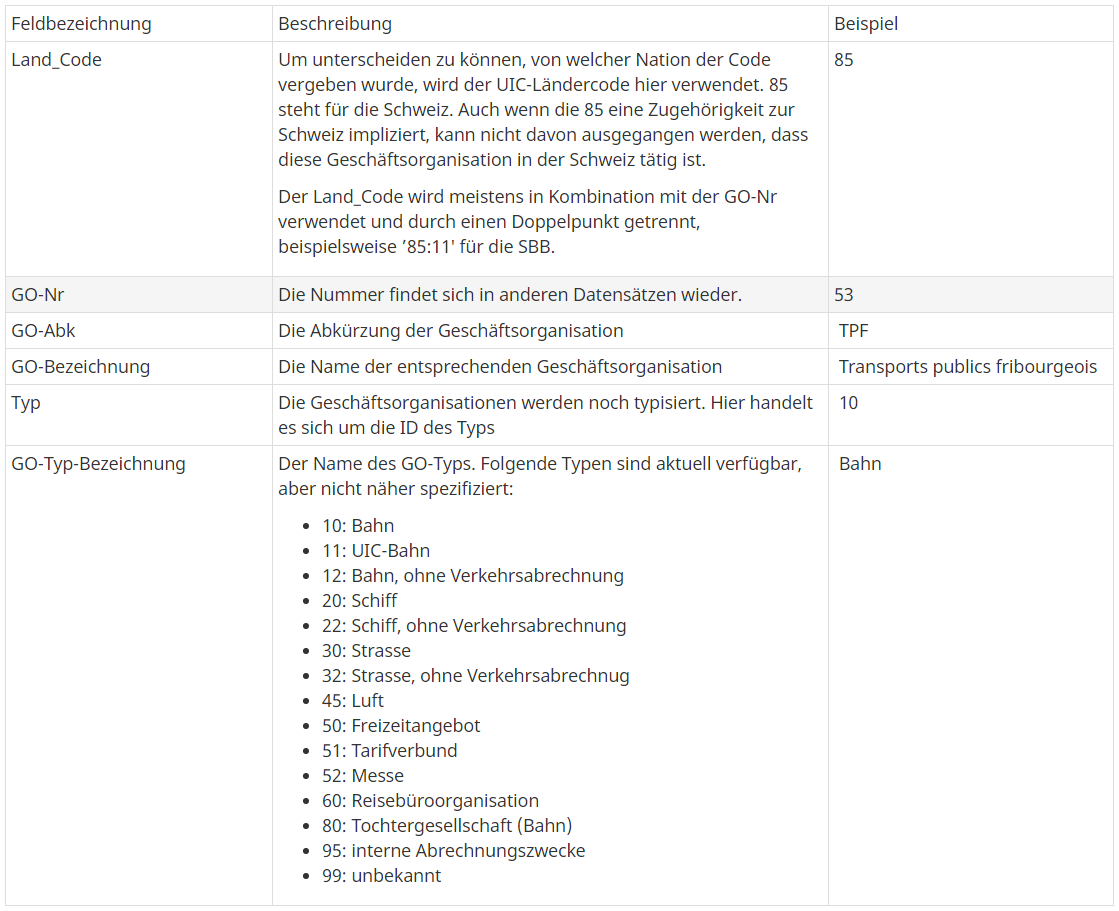
\includegraphics[width=12cm]{GOuebersicht.png}
	\caption{Beispiel einer Geschäftsorganisation mit Beschreibung der Attribute. \cite{geschaeftsorganisation}}
	\label{fig:Uebersicht Geschaeftsorganisationen}
\end{figure}
\subsubsection{Geschäftsorganisationen mit Echtzeit}
\label{Geschaeftsorganisationen mit Echtzeit}
Hierbei werden alle Geschäftsorganisationen erwähnt, die Echtzeitdaten liefern. Die Daten werden hier auch im Excel-Format zur Verfügung gestellt.

\begin{figure}[]
	\centering
	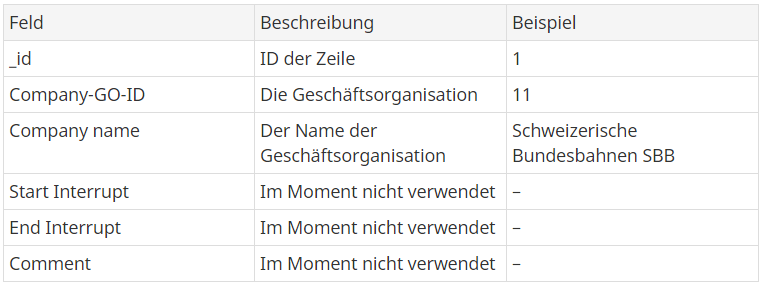
\includegraphics[width=12cm]{GO-Realtime.png}
	\caption{Beschreibung der Daten (Geschäftsorganisationen mit Echtzeit) anhand von einem Beispiel.\cite{geschaeftsorganisation-rt}}
	\label{fig:Uebersicht Geschaeftsorganisationen Echtzeit}
\end{figure}

\subsection{GA-HTA-Liste}
\label{GA-HTA-Liste}
In diesem Datensatz werden die Anzahl der General- (GA) und Halbtax-Abonnemente (HTA) pro Postleitzahl bereitgestellt mit dem dazugehörigen Erfassungsjahr. Diese Daten werden benötigt um Verkehrsmodelle zu verbessern, auf kantonaler und lokaler Basis.

\begin{figure}[]
	\centering
	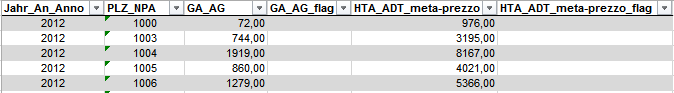
\includegraphics[width=12cm]{bspGA-HTA-Liste.png}
	\caption{Ausschnitt der Daten in einer GA-HTA-Liste  \cite{gahtaliste}}
	\label{fig:Beispiel GA-HTA-Liste}
\end{figure}
\begin{tabular}{|l|l|}  \hline
	Attribut & Beschreibung \\ \hline
	Jahr\_An\_Anno & Jahr des Stichdatums des Datenauszugs.  \\ \hline
	PLZ\_NPA & Vierstellige Postleitzahl gemäss Ortschaftenverzeichnis \\ \hline
	GA\_AG & Anzahl Generalabonnemente im Umlauf per Stichdatum. \\ \hline
	GA\_AG\_flag & Mittelwert Generalabonnemente, die weniger als 20Abos. \\ \hline
	HTA\_ADT\_meta-prezzo & Anzahl Halbtaxabonnemente im Umlauf per Stichdatum. \\ \hline	
	HTA\_ADT\_meta-prezzo\_flag & Mittelwert Halbtaxabonnemente, die weniger als 20Abos \\ \hline
\end{tabular}


\subsection{Bahnhofsliste (station list)}
\label{Bahnhofsliste}
Die Bahnhofsliste besteht aus zwei Dateien:
\begin{itemize}
	\item{\textbf{Station list}} - Hier sind alle Haltestellen der Schweiz enthalten, mit ID und Name.   
	\item{\textbf{Station geographic}} -Hier werden die Koordinaten für die Haltestellen zur Verfügung gestellt.
\end{itemize}
Die Dateien werden im CSV-Format bereitgestellt.
Die Station List entspricht die im HRDF-Format die "BAHNHOF"  Datei.\cite{bahnhofsliste}

\subsection{Abfahrts-/Ankunftsanzeiger (departure/arrival display)}%API
\label{sec:Abfahrts-/Ankunftsanzeiger}
Der Abfahrts- und Ankunftsanzeiger wird als Open Service API (application programming interface) zur Verfügung gestellt. Um die API zu benutzen muss man eine Haltestelle aus der Bahnhofsliste (station list) oder DiDok auswählen. Über diese API können mittels XML (Extensible Markup Language) Anfragen gestellt werden. Zusätzlich wird aber ein API-Key benötigt um Zugriff auf die API zu bekommen. Man verwendet sie für Haltestellenanzeiger. \cite{abfahrts-ankunftsanzeige}

\begin{figure}[]
	\centering
	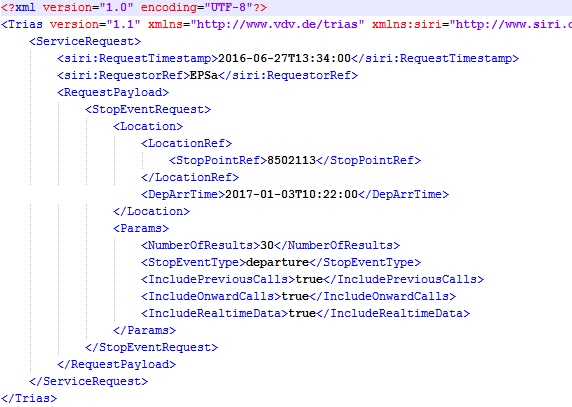
\includegraphics[width=12cm]{bspAbfrageAnkunftAbfahrt.png}
	\caption{Beispielcode einer Abfahrts-/Ankunft-Anfrage. Die Parameter, die Übergeben werden sind in schwarzer Schrift dargestellt.\cite{abfahrts-ankunftsanzeige}}
	\label{fig:Beispiel Anfrage Abfahrts-/Ankunftsanzeiger}
\end{figure}
\begin{tabular}{|l|l|}  \hline
	Parameter & Beschreibung \\ \hline
	8502113 & (StopPointRef) Haltestellencode Didok oder Bahnhofsliste   \\ \hline
	2017-01-03T10:22:00 & (DepArrTime)Ankunfts oder Abfahrtszeit \\ \hline
	30 & (NumberOfResults)Anzahl Resultate (maximal 40) \\ \hline
	departure & (StopEventType) entweder departure(Abfahrt) oder arrival(Ankunft) \\ \hline
	true & (IncludePreviousCalls)Haltestellen vor gesuchter Haltestelle mitliefern? \\ \hline	
	true & (IncludeOnwardCalls)Haltestellen nach gesuchter Haltestelle mitliefern? \\ \hline
	true & (IncludeRealtimeData)Sollen Echtzeitdaten mitgeliefert werden? \\ \hline
\end{tabular}

\subsection{Fahrtprognose (trip forecast)}%API
\label{sec:Fahrtprognose}
Wie auch beim Abfahrts- und Ankunftsanzeiger wird auch hier die Fahrprognose als Open Service API zur Verfügung gestellt.Ebnfalls wird auch hier über XML Anfragen gestellt und es wird auch ein API-Key benötigt.Sehr wichtig ist die JourneyRef(Fahrt-ID) diese muss bekannt sein und kann nicht über ein Sollfahrplan abgleitet werden, stattdessen wird sie über andere API-Request(TripRequest oder Ankunfts- und Abfahrtsanzeiger) abgeleitet.\cite{fahrtprognose}

\begin{figure}[]
	\centering
	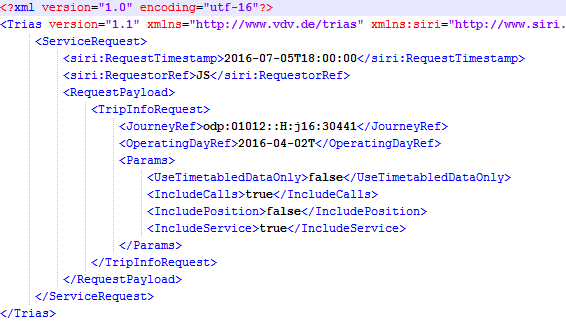
\includegraphics[width=12cm]{bspAbfrageFahrprognose.png}
	\caption{Beispielcode einer Fahrtprognose-Anfrage. Die Parameter, die Übergeben werden sind in schwarzer Schrift dargestellt.\cite{fahrtprognose}}
	\label{fig:Beispiel Anfrage Fahrtprognose}
\end{figure}

\begin{tabular}{|l|l|}  \hline
	Parameter & Beschreibung \\ \hline
	odp:01012::H:j16:30441& (JourneyRef)wird über andere Quellen bezogen/hergestellt   \\ \hline
	2016-04-02T & (OperatingDayRef)Betriebstag \\ \hline
	false & (UseTimetabledDataOnly)Infos zu Verkehrstagen ausgegeben werden? \\ \hline
	true & (IncludeCalls)Sollen Halte der Fahrt ausgegeben werden?   \\ \hline
	false & (IncludePosition)Aktuelle Position des Fahrzeugs mitliefern? \\ \hline	
	true & (IncludeService)Verkehrsmittelinformationen ausgeben? \\ \hline
\end{tabular}